\chapter{Idee future}
\section{Autenticazione delle chiamate API}
Al momento, nel progetto non è ancora stato implementato un metodo per autenticare le chiamate alle API definite. 
Questo passaggio è fondamentale per evitare che malintenzionati possano accedere, modificare 
o eliminare dati sensibili. Inoltre, l'autenticazione delle chiamate API è necessaria per conformarsi alle normative sulla 
protezione dei dati, come il GDPR, garantendo che le informazioni personali siano trattate con la massima riservatezza e sicurezza.
\section{Integrazione con Google Calendar}
Se l'utente acconsente a collegare il proprio account Google a RisUma, sarebbe opportuno sincronizzare automaticamente il calendario 
di RisUma con quello di Google ogni volta che viene fissato un colloquio. In questo modo, la gestione degli appuntamenti risulterebbe 
ancora più semplice ed efficiente. L'integrazione con Google Calendar permetterebbe agli utenti di visualizzare e gestire i propri 
appuntamenti direttamente dal loro calendario personale, senza dover accedere separatamente a RisUma. 
Ciò migliorerebbe significativamente l'esperienza utente, riducendo la probabilità di sovrapposizioni di 
appuntamenti e dimenticanze. Inoltre, l'integrazione potrebbe includere funzionalità avanzate come notifiche automatiche, 
promemoria via email o SMS e la gestione delle disponibilità, rendendo il processo di pianificazione dei colloqui più fluido 
e integrato con gli strumenti già utilizzati dagli utenti nella loro vita quotidiana.
\clearpage
\section{Miglioramento della visualizzazione mobile}
È necessario ottimizzare la pagina del sito per la visualizzazione su smartphone:
% Sezione dedicata alla visualizzazione del calendario
\begin{wrapfigure}{l}{0.45\textwidth}
    \centering
    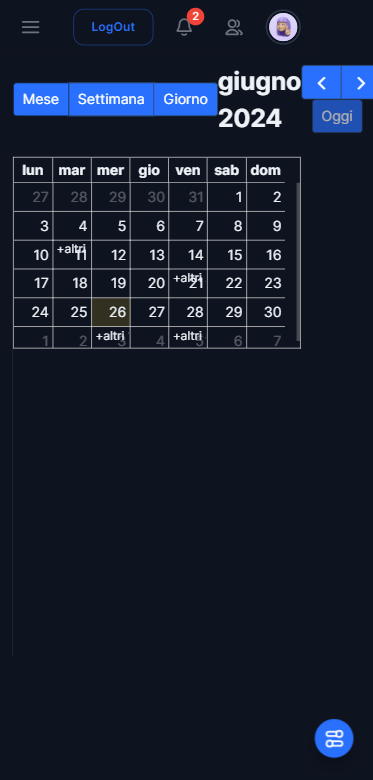
\includegraphics[width=0.45\textwidth]{Mobile/visualizzazioneCalendario.png} 
    \caption{visualizzazione calendario - mobile}
    \label{visualizzazione_calendario_mobile}
\end{wrapfigure}
\\
L'adattamento della pagina del sito alla visualizzazione mobile è fondamentale per garantire un'esperienza 
utente ottimale su tutti i dispositivi. In particolare, la visualizzazione del calendario \ref{visualizzazione_calendario_mobile} richiede una 
riprogettazione completa della barra di controllo superiore, magari introducendo una dropdown list per 
la scelta della visualizzazione e ridisponendo completamente le scritte e i pulsanti per muoversi nel calendario. 
Sarebbe utile implementare la funzionalità di swipe per passare da un mese all'altro senza dover necessariamente 
cliccare sui bottoni. Anche la visualizzazione del calendario deve essere ripensata per utilizzare meglio lo spazio verticale, 
estendendolo sia in altezza che in larghezza.
\clearpage
% Sezione dedicata ai popup
\noindent I due \texttt{Dialog} per i dettagli e la modifica di un evento, riportati nelle figure 
\ref{dettagli_meet_mobile} e \ref{modifica_meet_mobile},
si adattano già abbastanza bene a una 
visualizzazione da smartphone, ma si potrebbe sfruttare meglio lo spazio verticale aumentando lo spazio tra i vari 
componenti per rendere l'interfaccia ancora più pulita e godibile. 
\begin{figure}[H]
    \centering
    \begin{minipage}{0.45\textwidth}
        \centering
        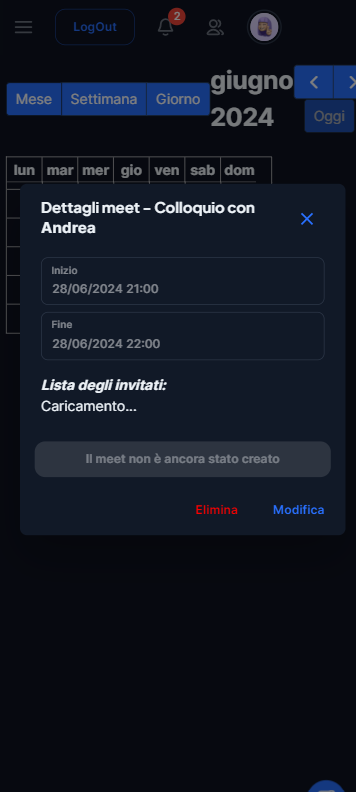
\includegraphics[width=\textwidth]{Mobile/popUpEvento.png}
        \caption{dettagli meet - mobile}
        \label{dettagli_meet_mobile}
    \end{minipage}
    \hspace{0.05\textwidth}
    \begin{minipage}{0.45\textwidth}
        \centering
        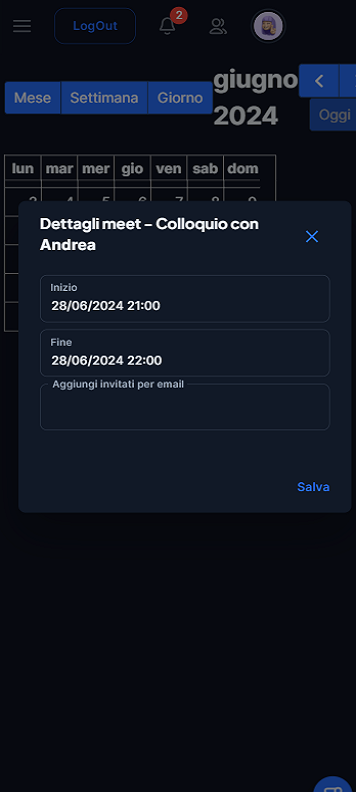
\includegraphics[width=\textwidth]{Mobile/popupModificaEvento.png}
        \caption{modifica meet - mobile}
        \label{modifica_meet_mobile}
    \end{minipage}
\end{figure}
\clearpage
% Sezione dedicata al picker di data e ora
\noindent Il \texttt{DateTimePicker} cambia automaticamente il tipo di visualizzazione in base al dispositivo utilizzato, 
il che elimina la necessità di ulteriori modifiche per questa specifica funzionalità. Viene riportato un esempio
nelle figure \ref{seleziona_data_mobile} e \ref{seleziona_ora_mobile}.
\begin{figure}[H]
    \centering
    \begin{minipage}{0.45\textwidth}
        \centering
        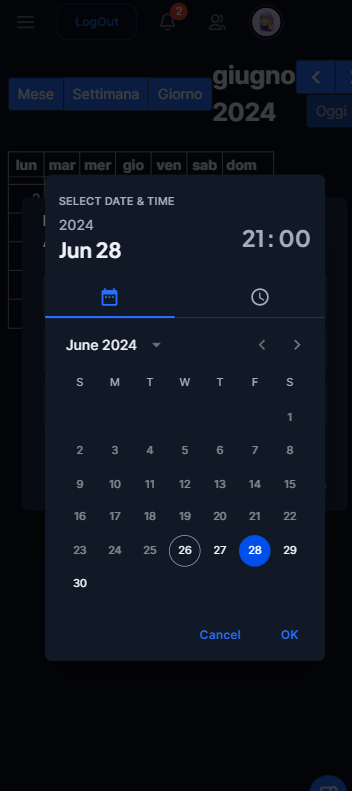
\includegraphics[width=\textwidth]{Mobile/selezionaData.png}
        \caption{seleziona data - mobile}
        \label{seleziona_data_mobile}
    \end{minipage}
    \hspace{0.05\textwidth}
    \begin{minipage}{0.45\textwidth}
        \centering
        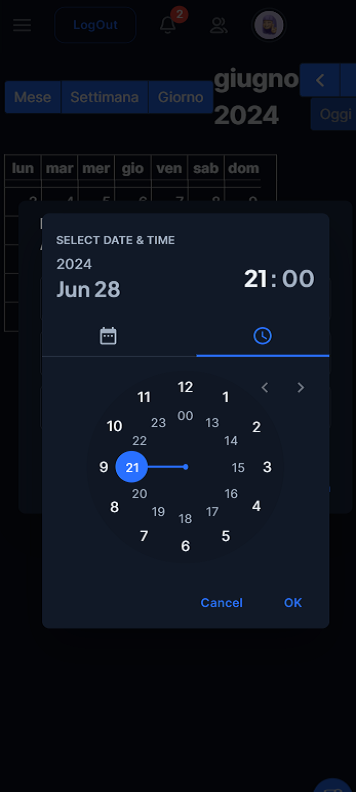
\includegraphics[width=\textwidth]{Mobile/selezionaOra.png}
        \caption{seleziona ora - mobile}
        \label{seleziona_ora_mobile}
    \end{minipage}
\end{figure}